\documentclass[border=10pt]{standalone}

\usepackage{siunitx}
\usepackage{amsmath}
\usepackage{pgfplots}
% TikZ Packages
\usepackage{tikz}
\usepackage{tkz-euclide}

\usetikzlibrary{angles, quotes, intersections, arrows, arrows.meta, babel, backgrounds, decorations, calc, intersections, patterns, positioning, shapes.geometric, patterns, patterns.meta, hobby}

\def\width{6}
\def\hauteur{6}
\def\N{100}

\definecolor{bluegray}{rgb}{0.4, 0.6, 0.8}

\newcommand{\drawPoint}[3]{
	\draw[ultra thin, dashed] (0,#2) -- (#1,#2);
	\draw[ultra thin, dashed] (#1,0) -- (#1,#2);
	\filldraw (#1,#2) circle (1pt) coordinate (P#3); 
}

\newcommand{\drawGrid}[4]{
	\draw[very thin, dotted] ($(#3, #4) - (0.5,0.5)$) grid ($(#1,#2) + (0.5,0.5)$);
%Draw axes
    \draw[-latex] ($(#3,0) + (-1,0)$) -- ($(#1,0) + (1,0)$) node[right] {$x$};
    
    \draw[-latex] ($(0,#4)+ (0,-1)$) -- ($(0,#2) + (0,1)$) node[above] {$y$};    
%Draw points in axes    
    \node at (-1.9ex,-1.9ex) {0};
    \foreach \x in {1,...,#1}
	{
		\node at (\x,-2ex) {\x};	
		\draw[thin] (\x, 0) -- (\x, -0.1); % Add a small dash	
	}
		\foreach \y in {1,...,#2}
	{
		\node at (-2ex,\y) {\y};
		\draw[thin] (0, \y) -- (-0.1, \y);			
	}
	
	
	\foreach \xprime in {#3, ..., -1}
	{
		\node at (\xprime,-2ex) {\xprime};	
		\draw[thin] (\xprime, 0) -- (\xprime, -0.1);			
	}
	
	\foreach \yprime in {#4, ..., -1}
	{
		\node at (-2ex, \yprime) {\yprime};		
		\draw[thin] (0, \yprime) -- (-0.1, \yprime);		
	}
}

\newcommand{\drawPosGrid}[2]{
	\draw[very thin, dotted] (-0.5, -0.5) grid ($(#1,#2) + (0.5,0.5)$);
%Draw axes
    \draw[-latex] (0,0) -- ($(#1,0) + (1,0)$) node[right] {$x$};
    
    \draw[-latex] (0,0) -- ($(0,#2) + (0,1)$) node[above] {$y$};    
%Draw points in axes    
    \node at (-1.9ex,-1.9ex) {0};
    \foreach \x in {1,...,#1}
	{
		\node at (\x,-2ex) {\x};	
		\draw[thin] (\x, 0) -- (\x, -0.1); % Add a small dash	
	}
		\foreach \y in {1,...,#2}
	{
		\node at (-2ex,\y) {\y};
		\draw[thin] (0, \y) -- (-0.1, \y);			
	}
	
}


\newcommand{\plainAxis}[2]{
  	\draw[-latex] (0,0) -- (#1,0) coordinate[label=right: $x$] (x);
  	\draw[-latex]  (0,0) -- (0,#2) coordinate[label=above: $y$] (y);
	\filldraw (0,0) circle (1pt) coordinate[label=below left: $O$] (o); 
}

\newcommand{\plainAxisFull}[4]{
  	\draw[-latex] (#3,0) -- (#1,0) coordinate[label=right: $x$] (x);
  	\draw[-latex]  (0,#4) -- (0,#2) coordinate[label=above: $y$] (y);
	\filldraw (0,0) circle (1pt) coordinate[label=below left: $O$] (o); 
}

\newcommand{\drawAxis}[4]{
%    \drawAxis{x}{y}{x'}{y'}
 \node at (-1.9ex,-1.9ex) {0};
\foreach \x in {1,...,#1}
	{
		\node at (\x,-2ex) {\x};	
		\draw[thin] (\x, 0) -- (\x, -0.1); % Add a small dash	
	}
		\foreach \y in {1,...,#2}
	{
		\node at (-2ex,\y) {\y};
		\draw[thin] (0, \y) -- (-0.1, \y);			
	}
	
	
	\foreach \xprime in {#3, ..., -1}
	{
		\node at (\xprime,-2ex) {-\xprime};	
		\draw[thin] (\xprime, 0) -- (\xprime, -0.1);			
	}
	
	\foreach \yprime in {#4, ..., -1}
	{
		\node at (-2ex, \yprime) {-\yprime};		
		\draw[thin] (0, \yprime) -- (-0.1, \yprime);		
	}

    \draw[-latex] (#3,0) -- (#1, 0) coordinate(x) node[right] {$x$}; % Draw x-axis
    \draw[-latex] (0, #4) -- (0, #2) coordinate(y) node[above] {$y$}; % Draw y-axis
}

\newcommand{\drawPosAxis}[2]{
%    \drawAxis{x}{y}{x'}{y'}
 \node at (-1.9ex,-1.9ex) {0};
\foreach \x in {1,...,#1}
	{
		\node at (\x,-2ex) {\x};	
		\draw[thin] (\x, 0) -- (\x, -0.1); % Add a small dash	
	}
		\foreach \y in {1,...,#2}
	{
		\node at (-2ex,\y) {\y};
		\draw[thin] (0, \y) -- (-0.1, \y);			
	}

    \draw[-latex] (0,0) -- (#1, 0) coordinate(x) node[right] {$x$}; % Draw x-axis
    \draw[-latex] (0,0) -- (0, #2) coordinate(y) node[above] {$y$}; % Draw y-axis
}

\newcommand{\drawAxisNoNums}[4]{
%    \drawAxis{x}{y}{x'}{y'}
    \draw[-latex] (#3,0) -- (#1, 0) coordinate(x) node[right] {$x$}; % Draw x-axis
    \draw[-latex] (0, #4) -- (0, #2) coordinate(y) node[above] {$y$}; % Draw y-axis
}

\newcommand{\drawPosAxisNoNums}[2]{
%    \drawAxis{x}{y}{x'}{y'}
    \draw[-latex] (0,0) -- (#1, 0) coordinate(x) node[right] {$x$}; % Draw x-axis
    \draw[-latex] (0,0) -- (0, #2) coordinate(y) node[above] {$y$}; % Draw y-axis
}

\def\centerarc[#1](#2)(#3:#4:#5){ \draw[#1] ($(#2)+({#5*cos(#3)},{#5*sin(#3)})$) arc (#3:#4:#5); }

\newcommand{\drawRectangle}[2]{
	\filldraw[black] (#1, #2) circle (1pt) ;
   	\draw[fill=blue, opacity=0.2] ($(#1,#2) - (0.5,0.5)$) rectangle ($(#1,#2) + (0.5,0.5)$) ;   
}
                
\newcommand{\drawRectangleCol}[4]{
	\filldraw[black] (#1, #2) circle (1pt) ;
   	\draw[fill=#3, opacity=#4] ($(#1,#2) - (0.5,0.5)$) rectangle ($(#1,#2) + (0.5,0.5)$) ;   
}
%
%\tikzset{
%	transition/.style = {
%		semithick,
%		->
%	},
%	every path/.style = {
%		transition, 
%		->, 
%		every node/.style={
%			font=\scriptsize, 
%			align=center
%		}
%	}
%}


\usetkzobj{all}

\usepackage{siunitx}

\begin{document}

	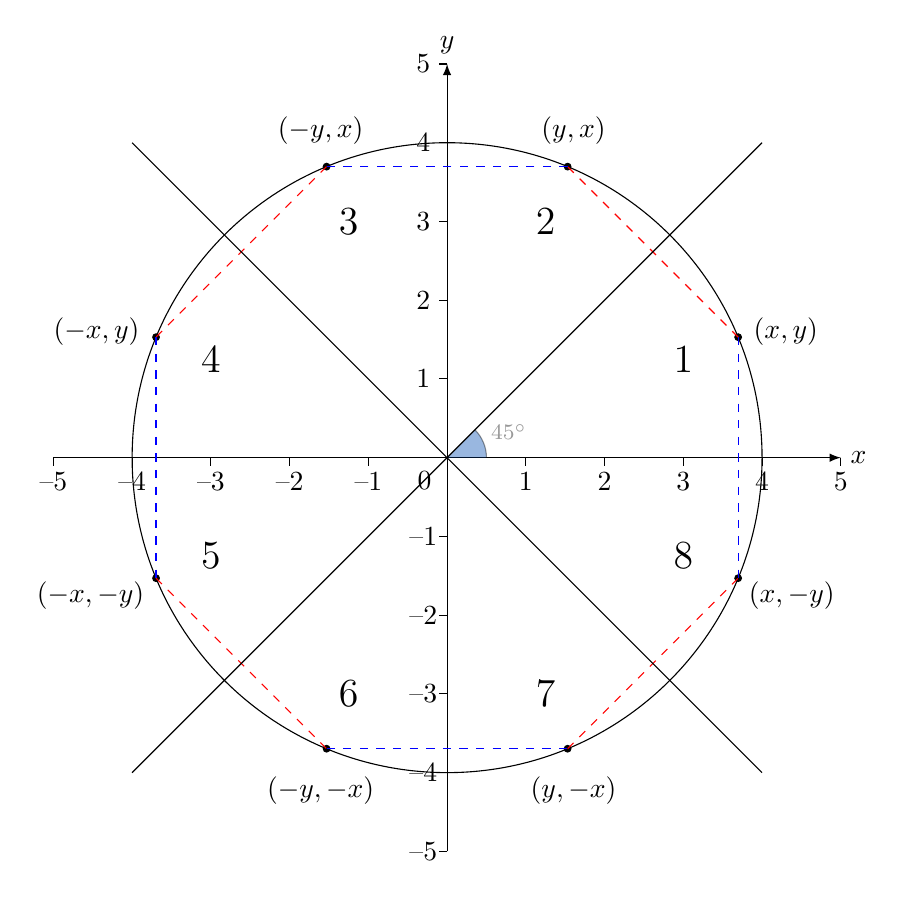
\begin{tikzpicture}[
		my angle/.style = {draw, fill=green!30!blue,
					opacity=0.4,
                   angle radius=5mm, 
                   angle eccentricity=1.7, 
                   font=\footnotesize} 
                   ]

%Define axis length and radius
    \pgfmathsetmacro{\axislength}{5}
    \pgfmathsetmacro{\radius}{4}

%Draw axes
    \drawAxis{\axislength}{\axislength}{-\axislength}{-\axislength}
    \coordinate (O) at (0,0);
    
%Draw circle
    \draw (O) circle[radius=\radius];
		
		
%Define paths 
	\path[name path=circle] (O) circle[radius=\radius];
    \path[name path=axis-x] (O) -- (\axislength, 0);
    \path[name path=axis-y] (O) -- (0, \axislength); 
    
    \path[name path=dichotomus1] (O) -- (45:\axislength);   

    
    \path[name path=bisector1] (O) -- (22.5:\axislength);   
	\path[name path=bisector2] (O) -- (67.5:\axislength); 
	\path[name path=bisector3] (O) -- (112.5:\axislength); 
	\path[name path=bisector4] (O) -- (157.5:\axislength);
	\path[name path=bisector5] (O) -- (202.5:\axislength);	 	
	\path[name path=bisector6] (O) -- (247.5:\axislength);	
	\path[name path=bisector7] (O) -- (292.5:\axislength);
	\path[name path=bisector8] (O) -- (337.5:\axislength);		 			 		

     
%Define the intersections
	\path[name intersections={of=circle and dichotomus1, by=A}];


	\path[name intersections={of=circle and bisector1, by=1}];
	\path[name intersections={of=circle and bisector2, by=2}];
	\path[name intersections={of=circle and bisector3, by=3}];    
	\path[name intersections={of=circle and bisector4, by=4}];
	\path[name intersections={of=circle and bisector5, by=5}];
	\path[name intersections={of=circle and bisector6, by=6}];    
	\path[name intersections={of=circle and bisector7, by=7}];
	\path[name intersections={of=circle and bisector8, by=8}];


%Points in circle  
	\draw[fill=black, draw=black] (1) circle (1.2pt) node [xshift=4ex, yshift=0.5ex] {$(x,y)$};
	\draw[fill=black, draw=black] (2) circle (1.2pt)	  node [xshift=0.5ex, yshift=3ex] {$(y,x)$};
	\draw[fill=black, draw=black] (3) circle (1.2pt)	 node [xshift=-0.5ex, yshift=3ex] {$(-y,x)$};
	\draw[fill=black, draw=black] (4) circle (1.2pt)	 node [xshift=-5ex, yshift=0.5ex] {$(-x,y)$};
	\draw[fill=black, draw=black] (5) circle (1.2pt)	 node [xshift=-5.5ex, yshift=-1.5ex] {$(-x, -y)$};
	\draw[fill=black, draw=black] (6) circle (1.2pt)	 node [xshift=-0.5ex, yshift=-3.5ex] {$(-y, -x)$};
	\draw[fill=black, draw=black] (7) circle (1.2pt)	 node [xshift=0.5ex, yshift=-3.5ex] {$(y, -x)$};  
	\draw[fill=black, draw=black] (8) circle (1.2pt)	 node [xshift=4.5ex, yshift=-1.5ex] {$(x, -y)$};


%Angle
	\pic[my angle, "$45^\circ$"] {angle = x--O--A};    
    
%Axis-mirrors    
	\draw[dashed, blue] (1) -- (8);
	\draw[dashed, blue] (2) -- (3);
	\draw[dashed, blue] (4) -- (5);
	\draw[dashed, blue] (6) -- (7);

%Bisector-mirrors    
	\draw[dashed, red] (1) -- (2);
	\draw[dashed, red] (3) -- (4);
	\draw[dashed, red] (5) -- (6);
	\draw[dashed, red] (7) -- (8);

%Octants
	\draw[thin] (-4,-4) -- (4,4);
	\draw[thin] (-4,4) -- (4,-4);
													
%Octant Points
	\draw[] (3,1.25)  node  {\Large{1}};
	\draw[] (1.25,3)  node  {\Large{2}};
	\draw[] (-1.25,3)  node  {\Large{3}};		
	\draw[] (-3,1.25)  node  {\Large{4}};

	\draw[] (-3,-1.25)  node  {\Large{5}};
	\draw[] (-1.25,-3)  node  {\Large{6}};
	\draw[] (1.25,-3)  node  {\Large{7}};		
	\draw[] (3,-1.25)  node  {\Large{8}};												
		
		
%%%%%%%%%%%%%%%%%%	
	

\end{tikzpicture}
	
\end{document}